\documentclass[conference]{IEEEtran}
\IEEEoverridecommandlockouts
% The preceding line is only needed to identify funding in the first footnote. If that is unneeded, please comment it out.
\usepackage{acronym}

\usepackage{esvect}

\acrodef{PSO}[PSO]{\emph{particle swarm optimisation algorithm}}
\acrodef{NN}[NN]{\emph{neural network}}
\acrodef{CPSO}[CPSO]{\emph{chaotic particle swarm optimisation algorithm}}
\acrodef{RNG}[RNG]{\emph{random number generator}}
\acrodef{CPRNG}[CPRNG]{\emph{chaotic pseudo-random number generator}}
\usepackage{cite}
\usepackage{amsmath,amssymb,amsfonts}
\usepackage{commath}
\usepackage{algorithmic}
\usepackage{graphicx}
\usepackage{textcomp}
\def\BibTeX{{\rm B\kern-.05em{\sc i\kern-.025em b}\kern-.08em
    T\kern-.1667em\lower.7ex\hbox{E}\kern-.125emX}}
\begin{document}

\title{Investigating Chaotic Particle Swarm Optimisation for Neural Network Training\\
}

\author{\IEEEauthorblockN{Quinton Weenink}
\IEEEauthorblockA{\textit{dept. Computer Science} \\
\textit{University of Pretoria}\\
Pretoria, South Africa \\
u13176545@tuks.co.za}
}

\maketitle

\begin{abstract}
Historically, particle swarm optimisation algorithms have successfully been applied to neural network training, often outperforming traditional gradient-based approaches. Studies have however shown that particle swarm optimisation algorithms do not scale very well, performing poorly on high-dimensional neural network architectures. This study aims to research the effect of using a chaotic particle swarm optimisation algorithm for neural network training. The resulting neural network's saturation and overfitting, as well as high-dimensional performance, will be investigated.
\end{abstract}

\begin{IEEEkeywords}
CPSO, NN, Chaotic
\end{IEEEkeywords}

\section{Introduction}
Chaotic maps are mathematical maps or evolution functions that exhibit some sort of chaotic behaviour. A \ac{CPSO} is a \ac{PSO} that makes use of a chaotic map as part of its implementation. There are different methods that all borrow from the same idea of applying the chaotic maps to the standard \ac{PSO} algorithm  \cite{pluhacek:cpso-iw}\cite{pluhacek:cpso-cprng-imp}. One of the best performing \ac{CPSO} implementations uses a \ac{CPRNG} for the random numbers required by the \ac{PSO}. The velocity for a particle is influenced by the chosen \ac{RNG}. Due to this, it can be hypothesised that the chosen \ac{RNG} could have a significant influence on the \ac{PSO}'s performance \cite{pluhacek:cpso-cprng-imp}.

While studies have been conducted on \ac{PSO} trained \ac{NN}s, as well as the performance of \ac{CPSO}s, none have been found to investigate the influence of \ac{CPSO} trained \ac{NN}. Saturation and overfitting, as well as high-dimensional performance of \ac{CPSO} trained \ac{NN}s have yet to be determined. This research aims to determine what influence the \ac{CPSO} has relative to the standard \ac{PSO} on \ac{NN} training.

In completing this research the understanding of \ac{CPSO}s as well as their effectiveness they have on \ac{NN} training will be improved. Additionally, this research aims to assist others when training \ac{NN}s with \ac{CPSO}s.

\section{Problem statement}
This research paper aims to determine whether the use of a \ac{CPSO} in \ac{NN} training increases performance over standard \ac{PSO} \ac{NN} training. Specifically, does the addition of a \ac{CPRNG} reduce saturation and overfitting in the trained \ac{NN}s? Additionally, does the use of a \ac{CPSO} improve on standard \ac{PSO} training for high dimensional \ac{NN} problems?

Investigating why or how the introduction of a chaotic map into a \ac{PSO} effects the saturation, overfitting, the high and low-dimensional performance of the trained \ac{NN}s is not the primary objective of this research.

\section{Literature survey}
Historically, \ac{PSO}s have been successfully applied to \ac{NN} training, sometimes outperforming traditional gradient-based approaches \cite{anna:saturation-psonn}\cite{anna:meas-sat-nn}. Studies have however shown that \ac{PSO}s do not scale very well, performing poorly on high-dimensional \ac{NN} architectures. This is as a result of high-dimensionality of the \ac{PSO}'s search space, primarily when a \ac{NN} with a high number of weights is used \cite{anna:saturation-psonn}. Critically, one must note that the research that was done on using \ac{CPSO}s to train \ac{NN}s have been quite limited and fail to indicate why and how certain chaotic maps are better or worse and why some were selected over others. Instead, one sees the use of \ac{CPSO} trained \ac{NN}s for specific research of narrow applications that do not indicate how they selected a map \cite{song:cpsonn}. This does not provide help for future research and in what situations \ac{CPSO}s should be used to train \ac{NN}s.

While the work by Pluhacek et al. has proven that \ac{CPSO}s offer better performance over standard \ac{PSO}s in a number of cases \cite{pluhacek:cpso-cprng-imp}\cite{pluhacek:ms-cpso}\cite{pluhacek:cpso-esb-chaotic}, it is not safe to conclude that \ac{PSO} \ac{NN} training will be improved in general. Additionally, research has not explored precisely when to use which chaotic map. Some research \cite{pluhacek:cpso-esb-chaotic}\cite{pluhacek:ms-cpso} attempts to solve this problem by using a multi-\ac{CPSO} or an ensemble of \ac{CPSO}s with the aim to design universally usable \ac{CPSO}s that will not suffer from some disadvantages of previous \ac{CPSO} designs \cite{pluhacek:pso-mutichaotic-ng}. This might also need to be investigated in order to increase performance regardless of the architecture size.

Reduced performance of \ac{NN}s has been hypothesised to be as a result of hidden layer saturation \cite{anna:saturation-psonn}\cite{anna:meas-sat-nn}. This prevents \ac{PSO} trained \ac{NN}s from performing regardless of the architecture size \cite{anna:meas-sat-nn}. Frequency distribution can be used to determine whether activation output is concentrated around the neurones asymptotic ends. This technique can indicate that there is saturation in the trained \ac{NN} \cite{anna:meas-sat-nn}.

\ac{NN} accuracy will be useful in determining whether \ac{CPSO} training has improved results over standard \ac{PSO} training as well as over gradient based training.

Overfitting results in a \ac{NN} that performs adequately on the training data but poorly on the generalisation. This is a result of the \ac{NN} mapping the training data too closely. Overfitting has been seen to reduce performance in \ac{NN}s trained by \ac{PSO}s \cite{vanwyk:overfitting-psoffnn}. Due to this one would need to explore sharing topologies and unbounded activation functions noting the effect that the \ac{CPRNG} has on performance.

\noindent While many studies have proven that \ac{CPSO}s have improved performance over standard \ac{PSO}s \cite{pluhacek:cpso-cprng-imp}\cite{pluhacek:ms-cpso}\cite{pluhacek:cpso-esb-chaotic}\cite{pluhacek:cpso-iw}\cite{pluhacek:lozi-cpso-mc} relatively little have studied the effects of training a \ac{NN} using a \ac{CPSO} and even less for problems of high-dimensionality. This gap in the field of \ac{CPSO}s should not go unstudied and the possibilities are exciting to investigate. While results do look positive for most applications of \ac{CPSO}s the results are applied to specific situations that may not be well suited for high-dimensional \ac{NN}s. Much still needs to be researched and investigated further in order to make sound assumptions about the possibilities such an algorithm would hold.



\section{Experimental Setup}
An \emph{experimental} research approach was decided on due to the unknown outcome of the suggested implementation. An experiment is required in order to make sound	evaluations on the research.

	\subsection{PSO}
	A \ac{PSO} is a machine learning algorithm where each particle in the population represents a possible solution to the optimisation problem \cite{anna:meas-sat-nn}. Each particle moves around the search space attempting to find the optimal solution with the influence of its neighbouring particles. The position for each particle iteration is calculated as follows.

	\begin{equation} \label{eq:1}
	\vec{x}_{i}^{\,t} = \vec{x}_{i}^{\,t-1} + \vec{v}_{i}^{\,t}
	\end{equation}

	\noindent Where:
	\begin{itemize}
		\item $x$ is the particle position vector in n-dimensions
		\item $v$ is the particle velocity vector, used to calculate the particles next position
		\item $t$ is the time increment
		\item $i$ is the particle number
	\end{itemize}
	\vspace{5mm}
	\noindent For each iteration of the algorithm, a new location of the particle is calculated based on its previous location and velocity vector as seen in (\ref{eq:1}).

	\begin{equation} \label{eq:2}
	\vec{v}_{i}^{\,t} = w . \vec{v}_{i}^{\,t-1} + c_1 . \vec{r}_{1}^{\,t} . (x_{pBest, i} - x_{i}^{t-1}) + c_2 . \vec{r}_{2}^{\,t} . (x_{nBest, i} - x_{i}^{t-1})
	\end{equation}

	\noindent Where:
	\begin{itemize}
		\item $c_1$ is the acceleration coefficient for the cognitive component
		\item $c_2$ is the acceleration coefficient for the social component
		\item $r_1$ and $r_2$ is a vector of random numbers
		\item $pBest$ is the personal best position of that particle
		\item $nBest$ is the best position found in that particles neighbourhood
	\end{itemize}
	\vspace{5mm}
	\noindent A particles social component, the third term in (\ref{eq:2}), requires $nBest$, the best neighbouring particles position. The set of neighbouring particles is determined by the topology used in the \ac{PSO}. Different topologies could influence the performance of the \ac{PSO}.

	Additionally, $ V_{max} $ velocity max, can be used as the limiter when calculating the particle's velocity in (\ref{eq:2}) ensuring that the particle stays inside search space. $ V_{max} $ might be required when applying \ac{PSO}s to \ac{NN}s and the effect the selected max should be evaluated.

	\subsection{CPSO}
	A \ac{CPSO} is a \ac{PSO} that makes use of a chaotic map as part of its implementation. The \ac{CPRNG} is one of the better performing implementations of the \ac{CPSO}. For this implementation, the \ac{CPRNG} will generate $ \vec{r}_{1} $ and $ \vec{r}_{2} $ used to calculate the particle's velocity in (\ref{eq:2}). The \ac{CPRNG} will use a chaotic map in order to calculate the generate the random number vectors.

	Chaotic map selection will be determined based on a number of factors that include the ability to allow variable dimensionality in order for to be applied to a \ac{PSO} for n-dimensions.

	Additionally, previous studies will be taken into account when selecting which of the applicable chaotic maps to apply. Such factors include high dimensional performance and scalability.

	\subsection{\ac{NN}}
	Typically, feedforward \ac{NN}s are comprised of neurons connected in layers. Signals travel from the input layer through the hidden layer(s) to the output layer \cite{anna:meas-sat-nn}. Each neuron is connected through a collection of weights to the neurons in the next layer.

	Back propagation is an often used training method for \ac{NN}s and makes use of forward propagation to generate the \ac{NN}'s output value(s). The weights are manipulated to train the network using the training error.

	\subsection{PSO trained NN}
	The goal of training a \ac{NN} with a \ac{PSO} is to find an optimal set of weights for the \ac{NN}. The \ac{NN}’s weights are represented by the \ac{PSO}'s dimensions. Each particle represents a \ac{NN} which could be a possible solution. The particle's fitness is determined by the accuracy of its resulting \ac{NN}.

	\subsection{Chaotic Maps and \ac{CPRNG}s}
	** Explain Chaotic maps here

	For this research, it was decided to implement the \ac{CPSO} using a \ac{CPRNG} due to previous papers indicating the better performance of such an implementation \cite{pluhacek:cpso-cprng-imp}.

	\subsubsection{Tinkerbell map}

	The Tinkerbell map (depicted in Fig. 6) is a two-dimensional complex discrete-time dynamical system given by (9)

	\begin{equation} \label{eq:3}
	X_{x+1} = X_n^2 - Y_n^2 + aX_n + bY_n
	\end{equation}
	\begin{equation} \label{eq:4}
	Y_{n+1} = 2X_nY_n cX_n + dY_n
	\end{equation}

\noindent with following control parameters: $ a = 0.9 $ and $ b = -0.6 $ used in , c = 2 and d = 0.5 [18].
	\begin{itemize}
		\item $x$ is the particle position vector in n-dimensions
		\item $v$ is the particle velocity vector, used to calculate the particles next position
		\item $t$ is the time increment
		\item $i$ is the particle number
	\end{itemize}
	\vspace{5mm}
	\noindent For each iteration of the algorithm, a new location of the particle is calculated based on its previous location and velocity vector as seen in (\ref{eq:3}).

	\subsubsection{Lozi map}

	\begin{equation} \label{eq:5}
	X_{x+1} = 1 - a \abs{X_n} + bY_n
	\end{equation}
	\begin{equation} \label{eq:6}
	Y_{n+1} = X_n
	\end{equation}

	\noindent Where:
	\begin{itemize}
		\item $x$ is the particle position vector in n-dimensions
		\item $v$ is the particle velocity vector, used to calculate the particles next position
		\item $t$ is the time increment
		\item $i$ is the particle number
	\end{itemize}
	\vspace{5mm}
	\noindent For each iteration of the algorithm, a new location of the particle is calculated based on its previous location and velocity vector as seen in (\ref{eq:3}).

	\subsubsection{Dissipative standard map}

	The Dissipative standard map is a two-dimensional chaotic map [15]. The Dissipative standard map is given in
Fig. 1. The map equations are given in Eqs. (\ref{eq:7}) and (\ref{eq:8}).

	\begin{equation} \label{eq:7}
	X_{x+1} = X_n + Y_{n+1} (mod 2\pi)
	\end{equation}
	\begin{equation} \label{eq:8}
	Y_{n+1} = bY_n + k sin X_n (mod 2\pi)
	\end{equation}

	\noindent The parameters constants used in this work are $ b = 0.6 $ and $ k = 8.8 $ will be used in (\ref{eq:8}) based on previous experiments \cite{pluhacek:cpso-cprng-imp}.


	\subsection{Executions and Iterations}
	In order to achieve viable results, each test will be run over 30 iterations. A control will be run for a standard \ac{PSO} trained \ac{NN}. The saturation, overfitting and high-dimensional performance of the control will need to be measured as a reference. The \ac{CPSO} will also be observed in the same manner. Each test will require testing of different variables and implementations. Such variables and include:
	\begin{itemize}
		\item Social topologies of the particles
		\item $c_1$ and $c_2$ acceleration coefficients for the cognitive and social components in (\ref{eq:2})
		\item $w$ inertia weight in (\ref{eq:2})
		\item $ V_{max} $ velocity max
		\item Chaotic map selection
		\item Number of input, hidden and output layer neurons for the \ac{NN}
		\item Activation functions of the \ac{NN}
	\end{itemize}


	\subsection{Research}
	In order to make sound assumptions about and the results, execution and manner in which these tests will be implemented much still needs to be researched and investigated.

	\subsection{Data sets}
	Selection of data sets will be based on previous studies that were done on \ac{PSO} training \ac{NN} performance. Additionally, the data sets that the experiment will be run on will be decided on based on applicability to the experiment, such as whether the data set will require a high weighted \ac{NN} in order to accurately map the solution. Well known and documented previous studies that show the resulting performance on that data set will also be desired in order to have a good and safe result set to use as the control.

	\subsection{Methodology for measuring performance}
	The training error, $E_T$ as well as the generalisation error, $E_G$ will be used in order to assess the resulting \ac{NN} accuracy. The training error is calculated as the mean squared error over the training set $D_T$ of size $P_T$ \cite{vanwyk:overfitting-psoffnn}.

\subsection{Some Common Mistakes}\label{SCM}
\begin{itemize}
\item The word ``data'' is plural, not singular.
\item The subscript for the permeability of vacuum $\mu_{0}$, and other common scientific constants, is zero with subscript formatting, not a lowercase letter ``o''.
\item In American English, commas, semicolons, periods, question and exclamation marks are located within quotation marks only when a complete thought or name is cited, such as a title or full quotation. When quotation marks are used, instead of a bold or italic typeface, to highlight a word or phrase, punctuation should appear outside of the quotation marks. A parenthetical phrase or statement at the end of a sentence is punctuated outside of the closing parenthesis (like this). (A parenthetical sentence is punctuated within the parentheses.)
\item A graph within a graph is an ``inset'', not an ``insert''. The word alternatively is preferred to the word ``alternately'' (unless you really mean something that alternates).
\item Do not use the word ``essentially'' to mean ``approximately'' or ``effectively''.
\item In your paper title, if the words ``that uses'' can accurately replace the word ``using'', capitalize the ``u''; if not, keep using lower-cased.
\item Be aware of the different meanings of the homophones ``affect'' and ``effect'', ``complement'' and ``compliment'', ``discreet'' and ``discrete'', ``principal'' and ``principle''.
\item Do not confuse ``imply'' and ``infer''.
\item The prefix ``non'' is not a word; it should be joined to the word it modifies, usually without a hyphen.
\item There is no period after the ``et'' in the Latin abbreviation ``et al.''.
\item The abbreviation ``i.e.'' means ``that is'', and the abbreviation ``e.g.'' means ``for example''.
\end{itemize}

\subsection{Figures and Tables}
\paragraph{Positioning Figures and Tables} Place figures and tables at the top and
bottom of columns. Avoid placing them in the middle of columns. Large
figures and tables may span across both columns. Figure captions should be
below the figures; table heads should appear above the tables. Insert
figures and tables after they are cited in the text. Use the abbreviation
``Fig.~\ref{fig}'', even at the beginning of a sentence.

\begin{table}[htbp]
\caption{Table Type Styles}
\begin{center}
\begin{tabular}{|c|c|c|c|}
\hline
\textbf{Table}&\multicolumn{3}{|c|}{\textbf{Table Column Head}} \\
\cline{2-4}
\textbf{Head} & \textbf{\textit{Table column subhead}}& \textbf{\textit{Subhead}}& \textbf{\textit{Subhead}} \\
\hline
copy& More table copy$^{\mathrm{a}}$& &  \\
copy& More table copy$^{\mathrm{a}}$& &  \\
\hline
copy& More table copy$^{\mathrm{a}}$& &  \\
copy& More table copy$^{\mathrm{a}}$& &  \\
\hline

\multicolumn{4}{l}{$^{\mathrm{a}}$Sample of a Table footnote.}
\end{tabular}
\label{tab1}
\end{center}
\end{table}

\begin{figure}[htbp]
\centerline{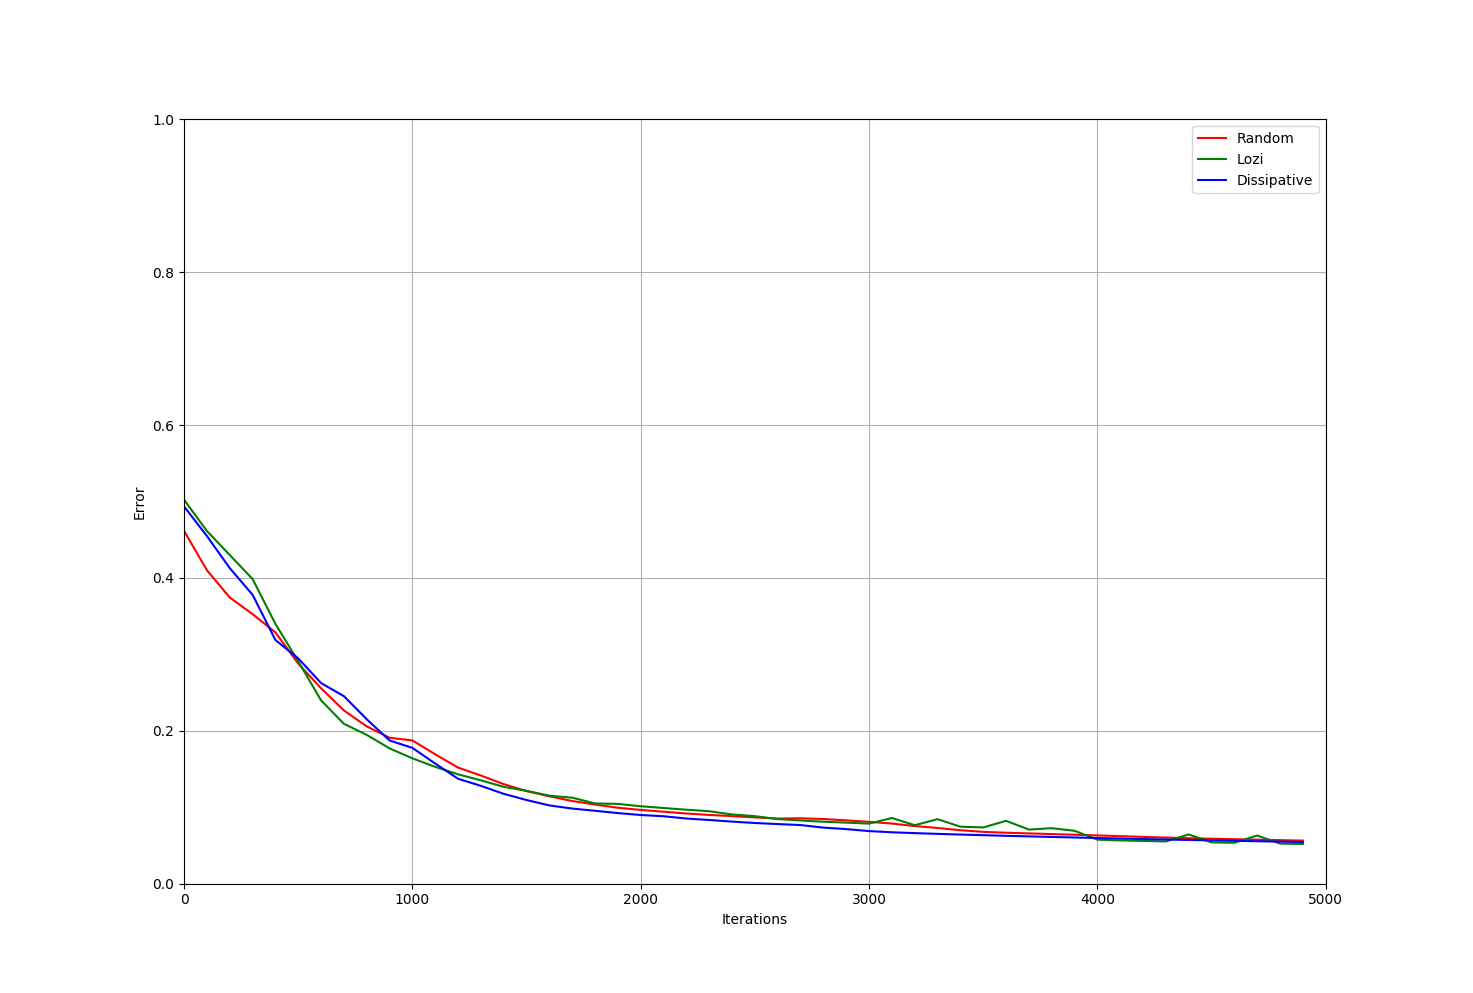
\includegraphics[width=100mm]{GlassResults.png}}
\caption{Example of a figure caption.}
\label{fig}
\end{figure}

Figure Labels: Use 8 point Times New Roman for Figure labels. Use words
rather than symbols or abbreviations when writing Figure axis labels to
avoid confusing the reader. As an example, write the quantity
``Magnetization'', or ``Magnetization, M'', not just ``M''. If including
units in the label, present them within parentheses. Do not label axes only
with units. In the example, write ``Magnetization (A/m)'' or ``Magnetization
\{A[m(1)]\}'', not just ``A/m''. Do not label axes with a ratio of
quantities and units. For example, write ``Temperature (K)'', not
``Temperature/K''.

\section*{Acknowledgment}

The preferred spelling of the word ``acknowledgment'' in America is without
an ``e'' after the ``g''. Avoid the stilted expression ``one of us (R. B.
G.) thanks $\ldots$''. Instead, try ``R. B. G. thanks$\ldots$''. Put sponsor
acknowledgments in the unnumbered footnote on the first page.


\nocite{*}
\noindent
\bibliographystyle{IEEEtran}
\indent
\bibliography{IEEEabrv,sbc-template}

\end{document}
